% Chapter 2

\chapter{Company Presentation} % Main chapter title

\label{Chapter2} % For referencing the chapter elsewhere, use \ref{Chapter2}

\lhead{Chapter 2. \emph{Company Presentation}} % This is for the header on each page - perhaps a shortened title


%----------------------------------------------------------------------------------------

\section{Presentation of Orange}
Orange, formerly France Telecom\cite{benilde2010portrait}, is a world-renowned French company specialized in the telecommunications sector. Orange has a rather eventful history due to multiple redemptions, but when France Telecom bought Orange PLC in August 2000, the group goes global. Orange has became the single brand of the group for the Internet, television and telephony (replacing Wanadoo, Itineris, Ola, Mobicarte ...). In 2006, Orange Business Services (OBS) appears to offer products and services to businesses and governments worldwide. At July 2013 that the France Telecom Group --- Orange takes the official name of \textbf{Orange}\cite{bertolus2003qui}.

\subsection{An International Operator}
Orange is the number three mobile operator and the number 1 ADSL television in Europe. The group is now present in 32 countries worldwide and strives to continue to deploy its foreign products and services . The operator carries much attention to the development of mobile services in Africa\cite{jaffre2005afrique} and the Middle East where it totals 88 million customers at 31 December 2013 (approximately 37\% of its customers). Some services Such "Orange Money" are deploying well abroad (8.9 million customers in Africa). Finally, since the arrival of 4G, Orange also invested in the coverage of European countries where customers are numerous (2 million customers in Poland and the UK in January 2014). Accordingly, Orange has 236 million customers worldwide (32 countries in 2014) while confused Service (76\% in mobile client) and employs 165000 people. The band has annual major case (about 41 billion euros in 2013).

%----------------------------------------------------------------------------------------

\section{Presentation of Orange Labs}
Innovation is a major growth lever for the Orange group. Research and development centers, also known as \textit{Orange Labs} form the group's innovation base. Today, 3,500 experts working within 18 Orange locations in 10 countries. In 2013, Orange continued its efforts in research and innovation by allocating 1.9\% of its turnover (780 million euros). Orange holds about 7,500 patents and apply 250 every year. Within the whole group, Orange employs 3700 people in research and development, and 200 PhD students and postdocs per year . The missions of research and development centers are:

\begin{itemize}
	\item The development of new quality products and services for the group,
	\item The release of new sources of growth with strong potential,
	\item The anticipation of technical and technological developments,
 	\item	The imagination of the solutions of the future with anticipation of long-term issues.
\end{itemize}

Orange is also widely involved in the many technical activities such as in standardization groups (eg 3GPP, IEEE or HGI) to be a major player in worldwide innovation.

%----------------------------------------------------------------------------------------
\section{Structure}
The company Orange is structured around various entities each with a specific role and specific occupations. Thus, the group consists of management entities, human resources management, communication, design, etc ... The entity Innovation, Marketing and Technologies (IMT) is responsible for giving a body to the operator in Internet era. Thus, IMT aims to digitize the operator in his close customer behavior, renewal of the various infrastructures and open the operation base station on the outside, based on innovation. This entity thus relies on innovation to differentiate themselves from the competition on marketing, to provide simple and reliable services and technologies and enrich its infrastructure.

IMT within various specialized research centers (Orange Labs Research), network (Orange Labs Networks), services (Orange Labs Products and Services), marketing (Technocentre), etc ... are responsible for delivering products and services focused on clients and their uses.

Composed of more than 3,000 people, Orange Labs Products and Services (OLPS) has overall technical responsibility for the products and services offered by Orange, the maintenance of implemented solutions in the world. Thus OLPS decomposes services that are more specific, such as SMA (SMart Access) which specializes in the domestic environment, SOFT which is specialized in the development of software components or UCE (Users and Customer Experience), which specializes in customer relationship. Each of these new services to decompose into smaller entities.

The chart below briefly presents how is structured Orange. There is more detailed for entities specialized in the design of new products and services, especially in the domestic field. The last level is the team working on the offer Smart Home Orange.

\begin{figure}[htbp]
	\centering
		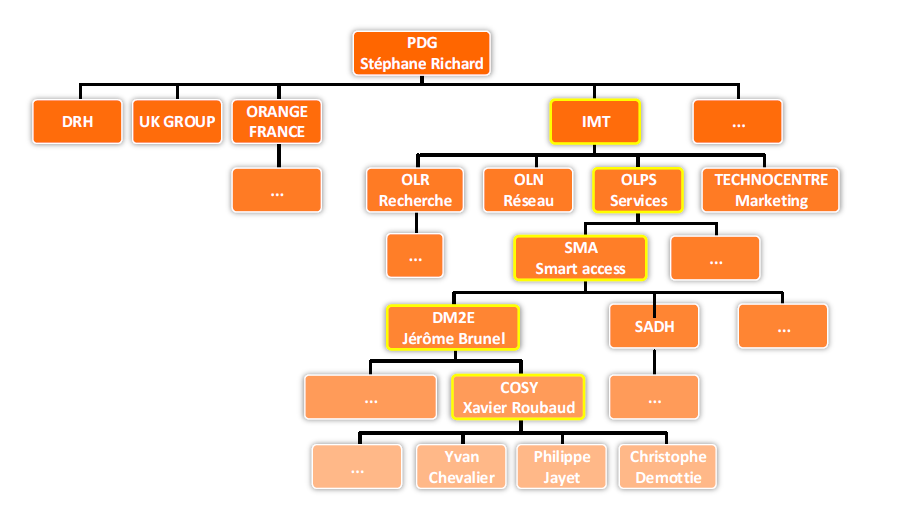
\includegraphics[width=9.5cm]{Figures/structureorange.png}
	\caption[Partial flow chart showing the structure of Orange]{Partial flow chart showing the structure of Orange}
	\label{fig:structure}
\end{figure}
%----------------------------------------------------------------------------------------
\section{Team CARE}

%----------------------------------------------------------------------------------------
